\documentclass[twoside]{AiTeX}



\title{PEV}
\author{A.L.K.}
\date{Diciembre 2021}
\begin{document}
%\datos{facultad}{universidad}{grado}{asignatura}{subtitulo}{autor}{curso}
\datos{Informática}{Universidad Complutense de Madrid}{Ingeniería informática}{Programación Evolutiva}{Memoria de la práctica 1}{Alejandro Barrachina Argudo \\ Adrià Carreras Bagur }{2023}
\portadaApuntes
\pagestyle{empty}
\tableofcontents
\pagestyle{empty}
\justify
\pagestyle{fancy}

\newpage

\chapterA{Capturas de funcionamiento}

\begin{figure}[H]
    \centering
    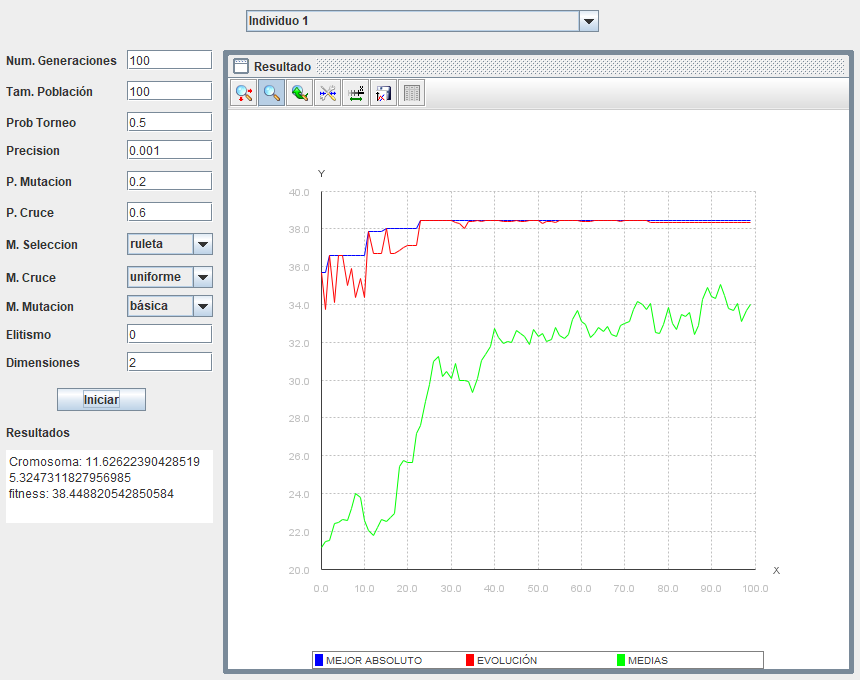
\includegraphics[width = \textwidth]{Images/Individuo1.png}
    \caption{Individuo 1}
    \label{fig:1}
\end{figure}

\begin{figure}[H]
    \centering
    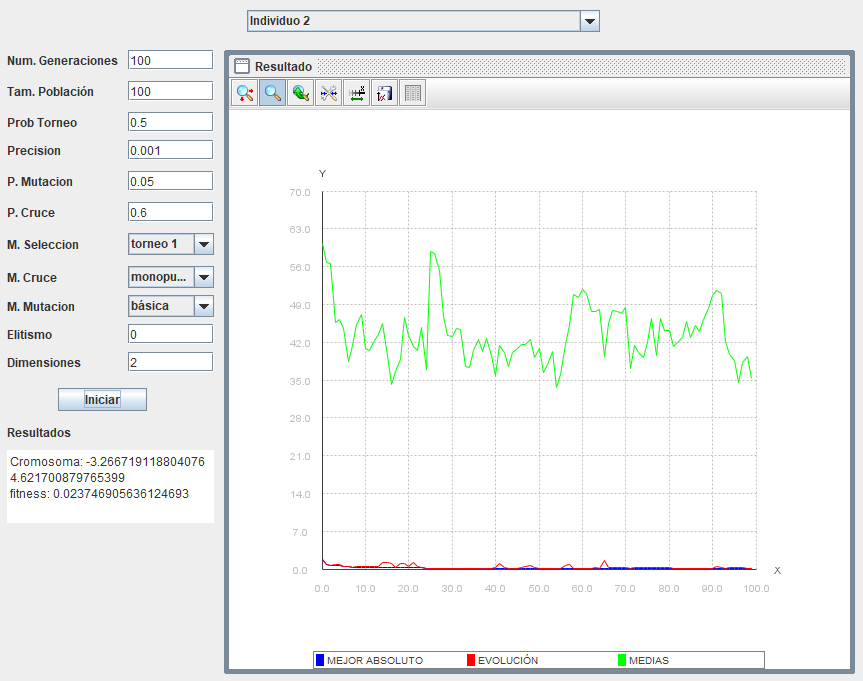
\includegraphics[width = \textwidth]{Images/Individuo2.png}
    \caption{Individuo 2}
    \label{fig:2}
\end{figure}

\begin{figure}[H]
    \centering
    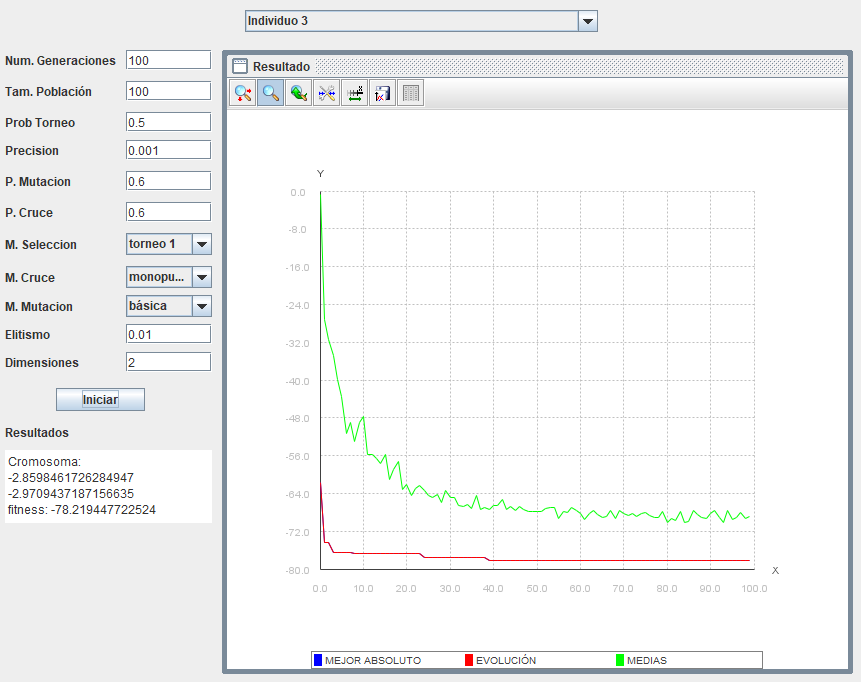
\includegraphics[width = \textwidth]{Images/Individuo3.png}
    \caption{Individuo 3}
    \label{fig:3}
\end{figure}

\begin{figure}[H]
    \centering
    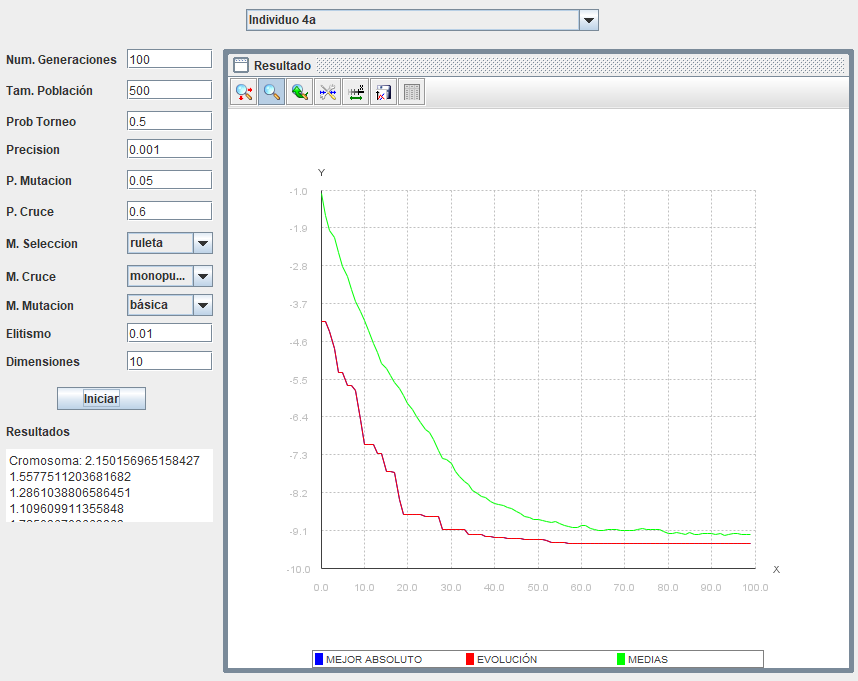
\includegraphics[width = \textwidth]{Images/Individuo4a.png}
    \caption{Individuo 4A}
    \label{fig:4a}
\end{figure}

\begin{figure}[H]
    \centering
    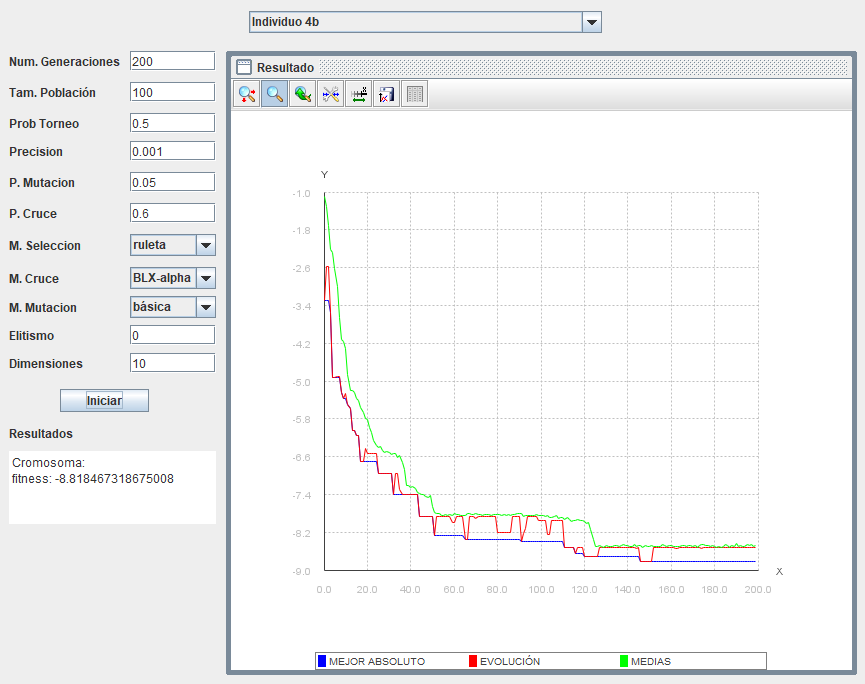
\includegraphics[width = \textwidth]{Images/Individuo4b.png}
    \caption{Individuo 4b}
    \label{fig:4b}
\end{figure}

\chapterA{Observaciones de la práctica, arquitectura del código y ejecución}

\section{Observaciones}

El método de selección que mejores resultados nos ha dado ha sido la selección por truncamiento, ya que al escoger solo los mejores individuos, siempre permite evolucionar mejor a la población.

El elitismo hace que la convergencia de la curva sea total entre el mejor absoluto y la evolución. Con valores altos de mutación ($>0.9$) da valores inconsistentes.

Podemos observar en la figura \ref{fig:4a} que el método de truncamiento para la selección provoca una evolución consistente y bastante convergente con el mejor absoluto incluso sin elitismo.

La primera función, en la figura \ref{fig:1}, nos sirve para ver como la mutación alta nos provoca unos cambios muy drásticos en la media de cada generación y cambios muy dispares en la línea de evolución.

Tanto en la figuras \ref{fig:1} y \ref{fig:4b} podemos ver que, aunque hace su trabajo, la selección por ruleta es la menos eficiente de las que tenemos en cuanto a evolución del individuo.

\section{Arquitectura}

Para mantener todo el código organizado, se usa la siguiente estructura de paquetes:

\begin{itemize}
    \item\textbf{go2:} paquete que engloba toda la práctica.
    \item\textbf{g02.cruces:} Paquete que reúne los cuatro cruces distintos bajo la interfaz Cruces.
    \item\textbf{g02.individual:} Paquete que contiene todos los individuos de las distintas funciones bajo la clase padre Individuo<T>.
    \item\textbf{g02.Selections}: Paquete para reunir las distintas selecciones usadas en la práctica bajo la clase padre Selection<T>, donde se encuentra las funciones para corregir el fitness.
    \item\textbf{g02.Ventana}: Paquete para la interfaz gráfica de la práctica y el método main.
\end{itemize}

Para una visión mas completa del proyecto, desde el navegador puede abrir el archivo G02/target/site/index.html

\section{Ejecución y compilación de la práctica}

Al ser un proyecto en maven se puede importar directamente desde eclipse con la opción de abrir proyectos del sistema de archivos.

Para compilar el proyecto solo hay que darle al botón de \textit{run} y debería instalar las dependencias necesarias. Si no fuera así se puede ejecutar el comando \textit{mvn install} para instalar todas las dependencias.

Así mismo, el proyecto se puede correr desde el propio eclipse usando el botón de \textit{run}, usando la configuración de \textit{aplicación java} y como clase principal g02.Ventana.ventana.

El archivo jar se encuentra en la carpeta P01/target/


\chapterA{Distribución de trabajo y conclusiones}

\section{Distribución}

Adrià ha hecho toda la GUI, parte de los cruces y parte de los individuos. Alejandro ha hecho la selección, parte de los cruces y parte de los individuos. La clase AlgoritmoGenetico se ha hecho entre los dos integrantes.

\section{Conclusiones}

En conclusión, el elitismo ayuda a un progreso más rápido de la evolución de una población siempre y cuando se use de forma moderada, ya que si no puede producir estancamientos. Los métodos de selección que mejor nos han funcionado han sido: torneos deterministas, truncamientos y estocástico. La mutación usada en valores exagerados nos ha causado problemas.


\end{document}
